\section{Background}
\label{sec:background}

Agent-to-business (A2B) coordination concerns the interaction through which agents acting for different organisations exchange proposals, delegate work and reach decisions. Consider a procurement agent evaluating a substitute part with a supplier. Logistics and compliance agents may join the discussion before a purchase is approved. Each organisation needs to identify the participants, recover the relevant conversation and inspect the evidence supporting the decision. Agent mediation increases the frequency and autonomy of these interactions; it does not introduce negotiation or cross-organisational accountability for the first time.


Existing agent interfaces address parts of this interaction but leave the shared record of proposals, authority and decisions to the application.
The Model Context Protocol (MCP) defines interfaces through which applications access tools and contextual resources~\citep{mcp2026spec}. Agent2Agent (A2A) defines agent cards, messages, tasks and multi-turn interactions~\citep{a2a2026spec}. These protocols support extended workflows, rather than only isolated request--response exchanges. Their use does not, however, determine the application's commercial terms, organisational authority or evidence-retention policy.

On the other hand, commerce protocols supply further parts of the interaction. The Universal Commerce Protocol (UCP) describes commerce capabilities and extensions, while the Agentic Commerce Protocol (ACP) specifies agent-mediated commerce interactions~\citep{ucpspec,acpspec}. AP2 provides mandates and verification procedures for delegated authorisation~\citep{ap2auth,ap2impl}. Table~\ref{tab:landscape} distinguishes these roles without treating their usual applications as limits on what can be built with them. Organisational identity can additionally be expressed through credentials whose issuers and claims the parties agree to trust~\citep{w3c2025vc}.

\noindent\begin{minipage}{\textwidth}
\centering\small
\captionof{table}{Interfaces relevant to A2B and their role in the present design.}
\label{tab:landscape}
\begin{tabularx}{\textwidth}{@{}P{2.2cm}LL@{}}
\toprule
Interface & Documented role & Role in the present design \\
\midrule
MCP & Tools and contextual resources & Access to an agent's operational systems \\
A2A & Agent discovery information, tasks and multi-turn messages & Execution interface between participating agents \\
UCP and ACP & Commerce interactions and capabilities & Related specifications for commercial workflows \\
AP2 & Delegated authorisation and mandate verification & Prior art for transaction-specific authority \\
AT Protocol & Account repositories, schemas and event distribution & Representation and distribution of coordination records \\
Agent Substrate & Sandboxed actor execution on Kubernetes & Candidate runtime for A2A services, not an implemented integration \\
\bottomrule
\end{tabularx}
\end{minipage}

The unresolved coordination problem is preserving the dependencies between proposals, checks, authorisations and outcomes across organisational boundaries. A successful compliance task does not by itself establish which offer version was checked. A valid mandate does not by itself establish that a later acceptance refers to that version. Separate logs may record both events without giving each party the evidence needed to verify their connection. If a proposal changes or a new agent joins, the relationship between earlier checks and the final decision must remain explicit. Otherwise, successful execution of the individual tasks can coexist with an unsupported commercial commitment. Figure~\ref{fig:a2b-evidence-gap} shows the problem: a compliance check on an earlier offer and acceptance of revised terms can coexist without evidence connecting the accepted version to that check, delegated authority or resource backing. The dotted links identify unresolved questions, not a proposed implementation.

\noindent\begin{minipage}{\textwidth}
\centering
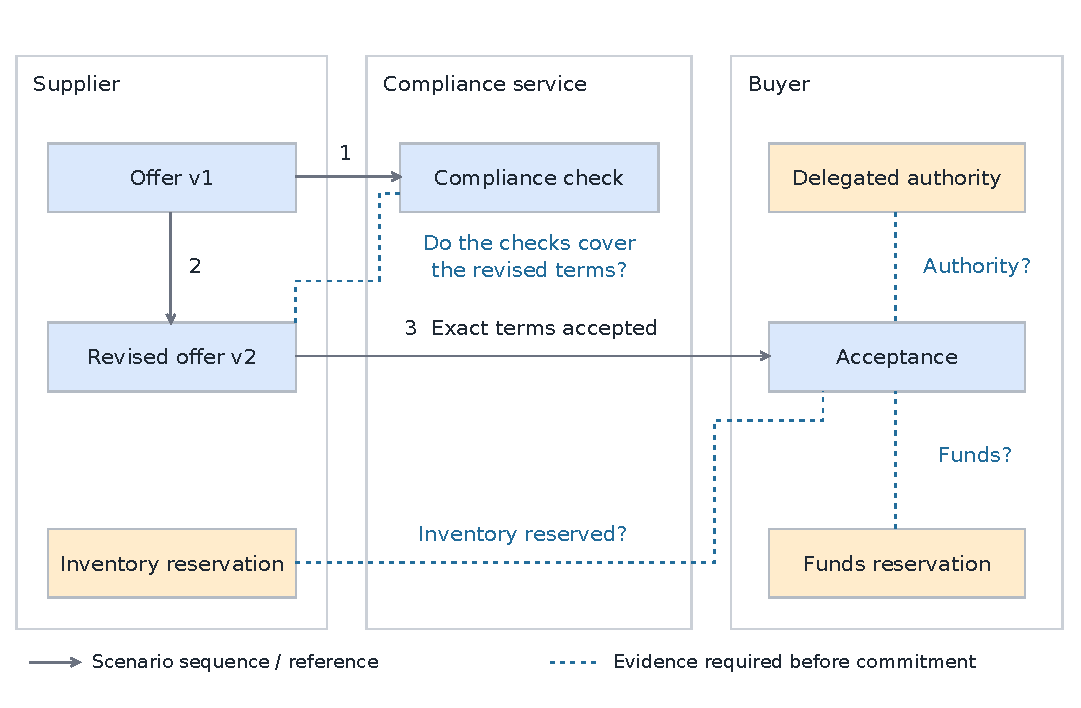
\includegraphics[width=\textwidth]{figures/a2b-evidence-gap.pdf}
\captionof{figure}{The A2B evidence gap across supplier, compliance service and buyer. An executed check does not establish an authorised commitment. Solid arrows show the original offer, its revision and acceptance of the revised terms. Blue boxes identify proposals, assessment and acceptance; amber boxes identify authority and resource evidence. Dotted links mark questions that task completion alone cannot answer: whether the assessment covers the accepted revision, the buyer has delegated authority and funds, and the supplier has reserved inventory. They denote required evidence, not completed checks.}
\label{fig:a2b-evidence-gap}
\end{minipage}

\subsection{What A2B requires: a coordination layer}
\label{sec:background-requirements}

Cross-organisational collaboration requires evidence that remains interpretable as proposals change and additional agents join. An auditor may need a supplier's offer, a compliance assessment and the buyer's decision, each produced by a different service. The relevant identity and trust policies must also be explicit. We use \emph{coordination layer} to mean the representation of these participants, requests, delegations and outcomes. Six requirements guide the proposal:
\begin{enumerate}[label=C\arabic*,leftmargin=*]
  \item \textbf{Verifiable identity:} An authorised recipient can verify the account key responsible for a record under an agreed identity-resolution and key-trust policy.
  \item \textbf{Shared, attributable record:} Requests, proposals and decisions are attributable through signed repository states, with verification material retained by each authorised party.
  \item \textbf{Published schemas:} Record types are defined once and validated by any participant, including one that joins a deal in progress.
  \item \textbf{Binding to exact content:} A response such as an acceptance identifies the precise version of the record it answers.
  \item \textbf{Discovery and fluid participation:} Participants can discover services and retrieve available prior records under agreed access and trust policies.
  \item \textbf{Controlled access and release:} Retrieval controls restrict access to sensitive records, while release policies govern which private information may enter outbound messages.
\end{enumerate}
Together, these requirements make the published basis of a decision inspectable across organisational boundaries. Commercial validity additionally requires shared business meaning. The parties must agree how a versioned domain profile defines quantities, prices and conditional charges, which settlement terms apply, and when confirmation creates an obligation under their framework agreement. Identical records do not ensure identical interpretations of that obligation. A valid decision must also fall within the agent's delegated authority and be consistent with the relevant resource reservations. Verification must therefore connect the record to agreed semantics, authority and resource state.
The method that follows specifies how these requirements are enforced during collaboration.

\subsection{The AT Protocol}
\label{sec:background-atproto}

The AT Protocol (atproto), developed for federated social applications, combines three traditions~\citep{kleppmann2024bluesky,atproto2026spec}: from the web, an open network of linked records; from peer-to-peer systems, self-certifying data and location-independent identity; and from data-intensive systems, an architecture in which canonical data is stored per account and changes flow through an event log to derived views. It was designed for a network with many parties, no shared operator, fluid participation and public accountability, which is the structural problem described in \cref{sec:background-requirements}. It separates the publication and verification of records from the services that host and interpret them.

\paragraph{Identity:} Each account has a decentralised identifier (DID)~\citep{w3c2022did} that resolves to verification keys and service endpoints, independently of where the account's data is hosted. \texttt{did:plc} resolves through a directory of operations signed by the account's own rotation keys; the directory operator cannot forge an identity, and the directory can be self-hosted by an organisation or consortium~\citep{plc2023spec}. \texttt{did:web} resolves a document served from a domain the holder controls, so its assurance rests on DNS and the web PKI and it keeps no history of key changes. Repository commits are signed by an account key. Historical verification requires trusted evidence of the key applicable at the time, rather than only the current DID document.

\paragraph{Records and schemas:} A Personal Data Server (PDS) hosts each account's repository, a Merkle search tree of typed records in which every node is content-addressed and every commit is signed by the owning DID. Lexicons define the types of records, service interfaces and event streams under reverse-DNS namespaced identifiers (NSIDs), so independent applications can adopt a common vocabulary without negotiating a bilateral format~\citep{atplexicon}. A Lexicon fixes the fields of, for example, an acceptance; whether that acceptance creates a commercial commitment remains an application decision.

\paragraph{Provenance and references:} An individual record is verified through its inclusion in a signed repository state~\citep{atprepo}. An AT URI identifies a record, and a content identifier (CID) identifies a specific version of its content. A \emph{strong reference} carries both, and replies cite their parents this way. A strong reference from an acceptance to the offer it answers therefore remains bound to that exact content when later offers revise the terms. Verification attributes a record to an account's key; it does not establish that the account holder may bind an organisation.

\paragraph{Distribution and indexing:} A relay crawls a configured set of PDSs and merges their commit streams into one event stream, the \emph{firehose}. Application views (AppViews) consume the firehose and build the reverse indexes that repositories cannot answer, such as every reply under a thread root, together with directories for discovery~\citep{atpsync}. Which repositories a relay crawls is a configuration choice. Each repository orders its own commits and each relay sequences its own stream, but no order across repositories is agreed by the participants.

\paragraph{Negotiation and commitment:} Negotiation and commitment have established foundations for A2B. Contract Net describes announcement, bidding and award, while FIPA ACL defines communicative acts including proposals and acceptance~\citep{smith1980contractnet,fipa2002acl}. UBL provides structured business documents~\citep{oasis2013ubl}. Causal references express dependencies between events, and transaction protocols distinguish agreement safety from progress under failures~\citep{lamport1978,graylamport2006}. The A2B challenge is to connect these foundations to discoverable agents and independently verifiable records throughout a changing interaction.

\Cref{tab:atproto-coordination} summarises what each mechanism contributes and what it leaves to the application. Three limits matter most for commerce. Repositories are mutable and the network does not guarantee retention, so each party must keep its own evidence. Relays provide neither complete coverage nor a global order of business events. The distribution model is public by design, with private data placed outside the repository abstraction~\citep{atproto2024roadmap}, so commercially sensitive exchanges need separate access control.

\begin{table}[htbp]
\centering
\small
\caption{AT Protocol coordination mechanisms and what each leaves to the application.}
\label{tab:atproto-coordination}
\begin{tabularx}{\textwidth}{@{}P{2.6cm}LL@{}}
\toprule
Mechanism & Coordination role & Left to the application \\
\midrule
Decentralised identifiers & Identify accounts across hosting domains; resolve keys and endpoints & Assurance depends on the DID method and key control; account identity does not establish corporate authority \\
Lexicon schemas & Shared types for announcements, proposals, responses and acknowledgements & Commercial meaning and enforcement of constraints \\
Signed repositories & Integrity of repository states and attribution of included records & Business validity; retention of historical states \\
AT URIs and CIDs & Bind an interaction to a specific version of another record & Availability of the referenced content and verification material \\
Relays & Distribute repository events from the PDSs they crawl & Complete coverage; ordering across repositories; confidentiality \\
Application views & Index records and relationships for discovery and queries & Completeness and interpretation of the indexed history \\
\bottomrule
\end{tabularx}
\end{table}

Access to information must also be distinguished from authority to disclose it~\citep{myers1997,robustdecl}. Restricting relay crawling does not secure every record, export or indexing route, and an agent authorised to send a message may still include private information. This boundary remains an application responsibility.

A solution must therefore do more than retain conversation history. It must bind a commercial decision to the exact terms, the agent's delegated authority and the resources reserved for that decision, while preserving the evidence each authorised party needs to inspect it. It must also support recovery without treating repeated execution as a new commitment and restrict disclosure without breaking necessary dependencies. These requirements define the conditions under which the coordination hypothesis can be assessed.
